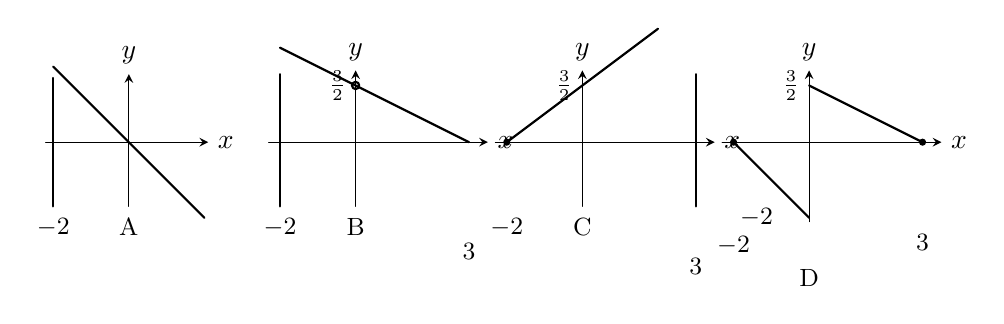
\begin{tikzpicture}[x=0.48cm,y=0.48cm,>=stealth,line cap=round,line join=round]
\tikzset{axis/.style={->,thin}, graph/.style={thick}, label/.style={font=\small}}
% 四幅图均为示意，除原图明示的截距/垂线外，不表达比例关系。
\begin{scope}[shift={(0,0)}]
  \draw[axis] (-2.2,0)--(2.1,0) node[right] {$x$};
  \draw[axis] (0,-1.7)--(0,1.8) node[above] {$y$};
  \draw[graph] (-2,2)--(2,-2);
  \draw[graph] (-2,-1.7)--(-2,1.7);
  \node[label] at (-2,-2.25) {$-2$};
  \node[label] at (0,-2.25) {A};
\end{scope}
\begin{scope}[shift={(6,0)}]
  \draw[axis] (-2.3,0)--(3.5,0) node[right] {$x$};
  \draw[axis] (0,-1.7)--(0,1.9) node[above] {$y$};
  \draw[graph] (-2,2.5)--(3,0);
  \draw[graph] (-2,-1.7)--(-2,1.8);
  \draw[graph] (0,1.5) circle (1.3pt);
  \node[label,left] at (0,1.5) {$\frac32$};
  \node[label] at (-2,-2.25) {$-2$};
  \node[label] at (3,-2.9) {$3$};
  \node[label] at (0,-2.25) {B};
\end{scope}
\begin{scope}[shift={(12,0)}]
  \draw[axis] (-2.3,0)--(3.5,0) node[right] {$x$};
  \draw[axis] (0,-1.7)--(0,1.9) node[above] {$y$};
  \draw[graph] (-2,0)--(0,1.5)--(2,3);
  \draw[graph] (3,-1.7)--(3,1.8);
  \fill (-2,0) circle (1.3pt);
  \node[label,left] at (0,1.5) {$\frac32$};
  \node[label] at (-2,-2.25) {$-2$};
  \node[label] at (3,-3.3) {$3$};
  \node[label] at (0,-2.25) {C};
\end{scope}
\begin{scope}[shift={(18,0)}]
  \draw[axis] (-2.3,0)--(3.5,0) node[right] {$x$};
  \draw[axis] (0,-2.1)--(0,1.9) node[above] {$y$};
  \draw[graph] (-2,0)--(0,-2);
  \draw[graph] (0,1.5)--(3,0);
  \fill (-2,0) circle (1.3pt);
  \fill (3,0) circle (1.3pt);
  \node[label,left] at (0,1.5) {$\frac32$};
  \node[label,left] at (-0.7,-2) {$-2$};
  \node[label] at (-2,-2.75) {$-2$};
  \node[label] at (3,-2.65) {$3$};
  \node[label] at (0,-3.6) {D};
\end{scope}
\end{tikzpicture}
